This section describes the exploration of the software/hardware co-design space.
The software side includes partitioning the program, determining the number of threads and the loop unrolling compiler optimization.
The hardware side is about finding out the best core composition that maximizes performance for a given partitioning.

\subsection{Thread Partitioning}

This section first starts with analyzing the impact of thread partitioning on performance.
Thread partitioning is about deciding how many threads to create and how to partition StreamIt filters into these threads.
To simplify this study, the default streaming partitioner is used to decide on how to allocate filters to cores which is based on simulated annealing.
%Define this
On the hardware side, two scenarios are considered:
the ``without composition scenario'' where there is exactly one core per thread and the ``with composition scenario'' where each thread receives between 1 and 15 cores.

Figure~\ref{fig:threadtrend} shows how performance varies under both scenarios as a function of the number of threads.
Regardless of how cores are composed it can be observed that all curves follow the same trend.
The optimal number of threads using core composition is very similar to the scenario without composition.
This important observation means that the optimal number of threads for a benchmark can be estimated independently from the hardware composition.
The system can therefore proceed in two stages: first determine the optimal number of threads and then decide on a core composition.

Figure~\ref{fig:threadtrend} also shows that the performance of most benchmarks starts to deteriorate passed a certain number of threads making it critical to not over-allocate threads.
This number of threads varies between benchmarks, thus it motivates the use of machine learning to decide the optimal number of threads to use.
Finally it is important to observe that executions without compositions always perform worse.
This demonstrates that composing cores is essential to obtain the best performance from a workload.


\subsection{Core Composition}

\begin{figure}[h]
  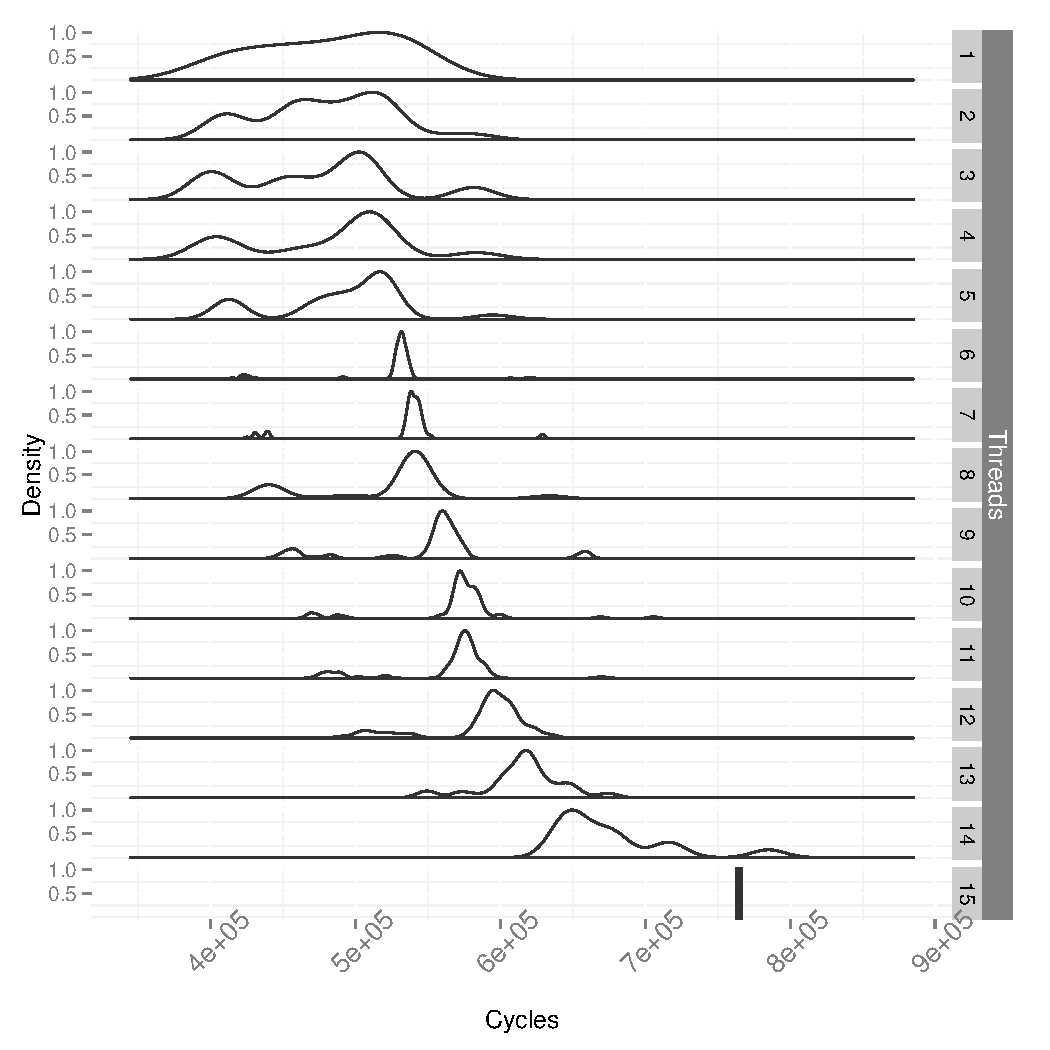
\includegraphics[width=1\textwidth]{streamit-paper/graphics/audiobeam_tots.pdf}
  \caption{Distribution of Audiobeam performance when modifying the amount of threads and compositions.}\label{fig:audiototal}
\end{figure}
Using core composition, the processor fuses a number of cores and associates them to a thread to increase single threaded performance.
Whilst this flexibility is advantageous, choosing the right amount of cores for a given thread is difficult due to the large number of possible configurations~\cite{gulati2008multitaskingdmc}.

Figure~\ref{fig:audiototal} shows how threading and composition affects performance for the \bench{Audiobeam} benchmark.
The curves represent the density distribution for different core compositions as a function of the number of threads.
The right hand side Y-axis represents the number of threads present in the current version of the benchmark normalized by the total number of points in the design space.
For each of the threaded versions the benchmark was ran using on average 100 different compositions.
The density curve for thread 15 is a single point as there exists only a single composition.

The variance of each of the curves represents the influence of composition on the benchmark's performance for a given number of threads.
For this benchmark the impact of core composition is actually very large for the best performing number of threads (1--5).
Interestingly, as more threads are used,  performance shifts worsens, echoing the results shown in the previous section.
Increasing the number of threads will increase communication between cores; which explains these results.
By fusing cores, this can reduce the stress of having multiple threads whilst still getting performance from having more cores being used.

\begin{figure}
  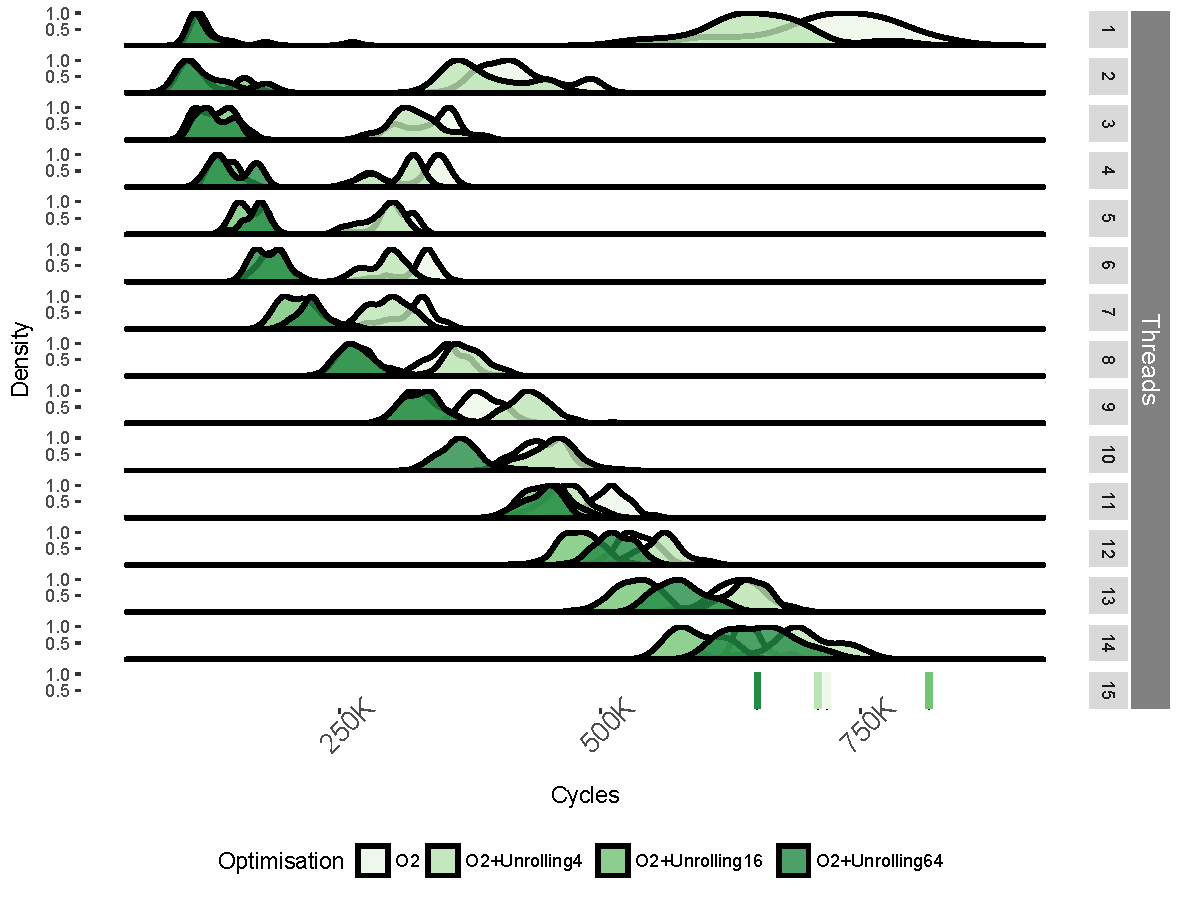
\includegraphics[width=1\textwidth]{streamit-paper/graphics/unrolled_fm.pdf}
  \caption{Distribution of FMRadio performance when modifying the amount of threads, composition and unrolling factor.}\label{fig:fmunroll}
\end{figure}

\subsection{Impact of Loop Unrolling}
In this section the impact of one compiler optimization is studied by focusing on loop unrolling.
Filters containing large amounts of loops potentially contain high degrees of instruction level and memory level parallelism.
Unrolling may increase the degree of parallelism which is advantageous to a wider fused processor.
Loop unrolling may also yield similar results to vectorization when vectorization may not easily be applied or available.

Figure~\ref{fig:fmunroll} presents an example of how loop unrolling affects performance on the \bench{FMRadio} benchmark.
The graph presents the same information as Figure~\ref{fig:audiototal} but with different executions of the benchmark when optimizing for speed and unroll factors 4, 16, and 64.
Figure~\ref{fig:fmunroll} shows that unrolling loops for \bench{FMRadio} can greatly improve performance.

Another observation is that the best execution times for each of the threaded versions when unrolling does not follow the same trend previously described.
The leftmost curve performance peaks at two threads whereas the rightmost peaks at five.
As the number of cores fused can now be greater we encounter a resource problem when increasing the number of threads, by a factor of 3x.
It is important to note that when increasing the amount of unrolling, the optimal thread shifts towards a smaller number.
This is due to the fact that more ILP can be extracted over TLP.
This example therefore demonstrates that whilst the optimal number of threads is independent of the number of cores there still exists trade-offs between the two.
This signifies that the amount of resources available to each thread must be taken into consideration before generating the program to balance the trade off between ILP and TLP.

\begin{sidewaysfigure}
 \centering
  \centering
    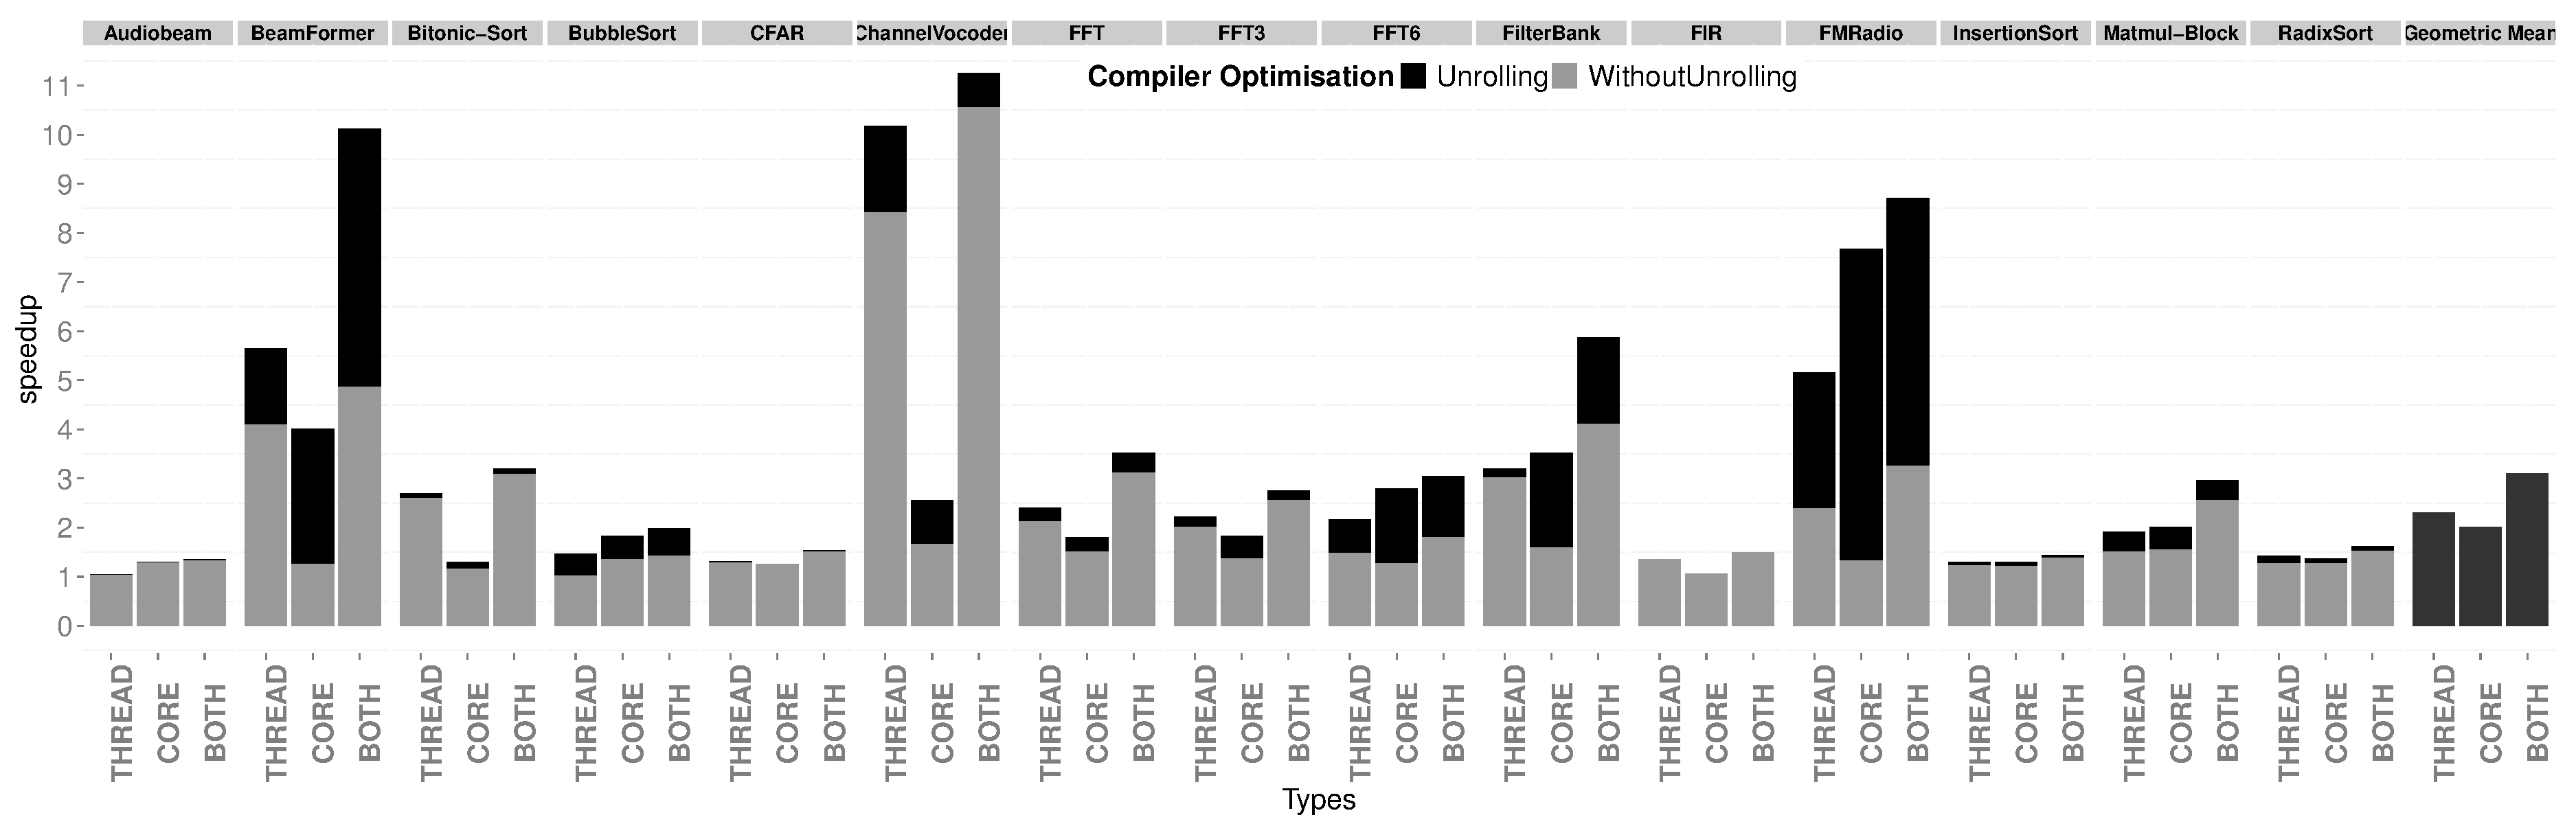
\includegraphics[width=1\textwidth]{streamit-paper/graphics/threadcompbench.pdf}
    \caption{Speedup obtained by choosing best core composition, best
      thread number and the combination of both optimisations. The baseline for the speedup measurement is single core, single thread execution using O2 compiler optimisations. Higher
      is better.}\label{fig:overviewhist}
\end{sidewaysfigure}

\subsection{Co-Design Space Best Results}

This section  presents the results of the entire co-design space exploration.
Figure~\ref{fig:overviewhist} characterizes how much of a performance increase is obtainable using a baseline of executing the benchmark on a single thread and single core without unrolling.
For each benchmark, the \textit{THREAD} bar represents the maximal speedup obtained by dividing the program into threads without fusing cores.
The \textit{CORE} bar represents the best speedup when the benchmark is executed in a single thread and fuse cores.
\textit{BOTH} represents the best speedup obtained for each benchmark using a combination of \textit{THREAD} and \textit{CORE}.
Finally, for each benchmark, these results were obtained for both an unrolled and not unrolled to compare how unrolling affects performance.
Figure~\ref{fig:overviewhist} shows that when loops are not unrolled, composing cores will not greatly improve performance.

When studying the geometric mean, without unrolling, finding the correct number of threads gives a speedup of 1.92 compared to 1.33 when using only core composition.
This changes when taking unrolling into account as the core compositions can be used more efficiently.
In this case, the speedup obtained from only composing cores is 13\% worse than using only threads. 
The unrolling demonstrates that the StreamIt programs must be modified to take advantage of the core composition.
Finally, it is important to note that whilst finding the optimal thread mapping is better than the best composition, the best performance is always obtained through a combination of both optimizations. 

\subsection{Summary}

This section demonstrated that each parameter has a large effect on the performance of the workload.
Regardless of using core composition or not, there exists for each benchmark an optimal number of threads.
Unrolling is effective at exposing more opportunities for composition due to increased ILP but there is a balance to strike between extracting ILP and TLP.
Figure~\ref{fig:overviewhist} shows there is a 3x benefit (overall) by automating the partitioning of both the software (threads) and hardware (cores).

